\subsection{Approach}
\label{evalapproach}
The evaluation is restricted to an evaluation of topic clustering ability, on which the thesis is focused. Comparing the topic models LDA and HMDP to the graph-clustering algorithm MCL extrinsically relies on a grouped gold standard.
Ideally, evaluation should base on a large dataset. However, we were unable to find a sufficient dataset with gold standard grouping and annotating a large dataset in its entirety is infeasible in the restricted timeframe of the thesis. Thus, a subset of 100 of 6195 comments contained in dataset \#3 was annotated and grouped into five broad topic clusters. The annotation scheme was as follows. Five comments with clearly distinct topics were chosen as seed comments. Then, random samples of the entire set were taken. If a comment was clearly about the same topic as one of the seed comments, it was grouped to it. If the topic could not be determined directly, e.g. for a short comment such as "This is a great idea", additional information in form of the conversational thread was taken into account. If, based on this additional info, the topic was one of the seeds comments topics, the comment was grouped to the seed comment. Otherwise a new sample was taken. \par
All models were trained on only the 100 grouped comments as well as on the entire dataset. The 100 annotated comments were in both cases used for evaluation based on the metrics BCubed Recall, BCubed Precision and BCubed F-measure, which were used to compare LDA and MCL in \cite{DBLP:conf/ecir/AkerKBPBHG16}. The BCubed measures fulfill all four constraints for extrinsic cluster evaluation metrics set in \cite{DBLP:journals/ir/AmigoGAV09}. These are cluster homogeinity, completeness, rag bag which attributes for noisiness and size vs. quantity \cite{DBLP:journals/ir/AmigoGAV09}. Recall and precision are calculated on a per item basis and then averaged. While arbitrary weights for datapoints are possible, each one is given the same weight in our evaluation. Precision and recall are defined according to \cite{Bagga98algorithmsfor} as follows. Let $N$ be the number of comments, $c_i \in C^{t_i} = \{c \in C|t_i = \argmax_{t \in T} P(t|c)\}$ be a comment and its associated topic cluster and $G_i$ the gold standard cluster of comment $c_i$.
\begin{definition}{BCubed Precision}
\begin{align}
\text{Precision} &= \sum_{i=1}^N \frac{\text{Precision}(c_i)}{N} \\
\text{Precision}(c_i) &= \frac{|\text{correctly clustered comments in }C^{t_i}|}{|C^{t_i}|}
\end{align}
\end{definition}
\begin{definition}{BCubed Recall}
\begin{align}
\text{   Recall} &= \sum_{i=1}^N \frac{\text{Recall}(c_i)}{N} \\
\text{   Recall}(c_i) &= \frac{|\text{correctly clustered comments in }C^{t_i}|}{|G_i|}
\end{align}
\end{definition}
F-measure is then calculated according to \cite{Chinchor:1992:MEM:1072064.1072067}.
\begin{definition}{F-measure}
\begin{equation}
F_\beta = \frac{(\beta^2 + 1) \cdot \text{Precision} \cdot \text{Recall}}{\beta^2 \cdot \text{Precision} +\text{Recall}}
\end{equation}
$\beta > 1$ favors recall, $\beta = 1$ calculates the harmonic mean and $\beta < 1$ favors precision.
\end{definition}
For evaluation using only the 100 annotated comments for training, $\beta = 1$ and the number of inferred and gold standard clusters are chosen to be equal. For the MCL, such restrictions were achieved based on empirical evaluation of different inflation parameters. In the setting where all comments are clustered, on the other hand, $\beta = 0.5$ is chosen, since the number of inferred groups differs significantly from the number of groups in the gold standard, which is necessary for a natural evaluation. Therefore, it is expected that comments, which where grouped together in the coarsely grouped gold standard, are grouped in multiple, more fine-granulated groups. Thus, a higher number of false negatives \footnote{Comments clustered together by gold standard but not the model.} is expected which is penalized in recall. Precision is given a higher weight with $\beta = 0.5$ as advised in \cite{Chinchor:1992:MEM:1072064.1072067}, based on the notion that clustering comments dissimilar by topic together should be penalized stronger than separating topics into more fine-granulated clusters. \par
In addition, both topic models are compared using Perplexity. 30\% of documents are held-out for testing in the corpus D$_{\text{test}}$ and the model is trained on the other 70\% of documents in corpus D$_{\text{train}}$. Perplexity describes, how likely new observations are on the held-out documents with the trained model which tests the hypothesis of the generative process of document creation. Lower perplexity indicates a higher likelihood of new documents and better performance \cite{DBLP:phd/dnb/Kling16}.
\begin{definition}{Perplexity}
\begin{equation}
\text{perplexity}(\text{D}_{\text{test}}) = \text{exp}\left(-\frac{\sum_{j=1}^M\sum_{i=1}^{N_i}\text{log}p(w_{ji})}{\sum_{j=1}^MN_i}\right)
\end{equation}
\end{definition}
Evaluation of the HMDP includes an evaluation of context space influence carried out by inspection of context space weights. This provides information about the indicativeness of the considered forms of metadata.
\subsection{Results}

\subsubsection{MCL}
In order to find out whether the results reported in \cite{DBLP:conf/ecir/AkerKBPBHG16} translate well for summarizing comments of multiple articles, the approach in \cite{DBLP:conf/ecir/AkerKBPBHG16} was replicated and the MCL applied on all three datasets. While algorithm and graph build-up are generally fast on the two smaller datasets, their combination took 1h35m on dataset \#3. Different inflation parameter values, which can range from 1.2 for a coarse clustering to 5.0 for a fine granulated clustering, were tried out.
\begin{table}[H]
\centering
\caption{Distribution of the number of threads contained in clusters found on dataset \#3 by the MCL as replicated from \cite{DBLP:conf/ecir/AkerKBPBHG16} for different inflation parameters.}
\begin{tabular}{||l||c|c|c||}
\hline
 & 2.0 & 1.2 \\
\hline
No. of topics & 923 & 574 \\
Standard deviation & 0.24 & 1.78   \\
Minimum & 1.0 & 1.0 \\
25\%-Quantile & 1.0 & 1.0 \\
50\%-Quantile & 1.0 & 1.0 \\
75\%-Quantile & 1.0 & 2.0 \\
Maximum & 7.0 & 8.0 \\
\hline
\end{tabular}
\end{table}
The starting value was set to 2.0 as advised by van Dongen in \footnote{\url{https://micans.org/mcl/}}. The MCL identified 923 clusters for 6195 comments. Upon inspection of the clustering structure, it became apparent that almost all clusters contained only a single thread. Inflation parameter 1.2 still resulted in 574 clusters and a median number of one thread per cluster. This version of the MCL generally appears to overfit the thread structure of comments through thread-relationship measure. In contrast, the version presented in this thesis, which only uses cosine similarity based on TF-IDF vectors and thread-relationship of two comments for graph build-up, finds 142 clusters for inflation parameter 2.0 and results in a more natural clustering. Therefore, this version is meant with 'MCL' for the remaining parts of the thesis.

\subsubsection{Comparison of HMDP, LDA and MCL}
\label{comparison}
\begin{table}[h]
\centering
\caption{Performance on 100 gold standard comments. The number of topics in topic models was restricted to 5 and the inflation parameter of the MCL was set to 1.55 to obtain 5 groups corresponding to the gold standard.}
\begin{tabular}{||l||c|c|c||}
\hline
 & HMDP & LDA & MCL \\
\hline
Precision & 0.44 & 0.34 & 0.38 \\
Recall & 0.65 & 0.49 & 0.69 \\
F$_{1}$-measure & 0.52 & 0.40 & 0.49 \\
\hline
\end{tabular}
\end{table}
When compared only on the 100 gold standard comments, HMDP and MCL outperform the baseline LDA significantly. Furthermore, MCL has a slightly higher recall, whereas HMDP provides a higher precision. Combining both measures in the F$_1$ measure, results in HMDP having an edge over the MCL.
\begin{table}[h]
\centering
\caption{Performance on dataset \#3 using 100 gold standard comments for evaluation. Here, F$_{0.5}$ was calculated as outlined above. The number of topics was restricted to 80 in LDA and HMDP and the inflation parameter i=1.808 used in the MCL to obtain 80 clusters. In both topic models, words occuring at least 20 times were kept.}
\begin{tabular}{||l||c|c|c||}
\hline
 & HMDP & LDA & MCL \\
\hline
Precision & 0.78 & 0.67 & 0.5 \\
Recall & 0.27 & 0.2 & 0.64 \\
F$_{0.5}$-measure & 0.57 & 0.45 & 0.52 \\
\hline
\end{tabular}
\end{table}
When trained on all comments, the results differ greatly from before. HMDP and MCL again outperform LDA. HMDP has high precision, followed by LDA and MCL with significant distance each. Recall, however, is high for the MCL but generally lower for HMDP and LDA. The HMDP again performs better than LDA in terms of recall. In terms of F$_{0.5}$-measure, the HMDP can be made out as the best performing model.
To make sense of the drastic difference between the results obtained in both settings, we want to take a closer look at the clustering structure.
\begin{table}[H]
\label{clusterstruc}
\centering
\caption{Distribution of the number of comments contained in clusters found on dataset \#3.}
\begin{tabular}{||l||c|c|c||}
\hline
 & HMDP & LDA & MCL \\
\hline
Standard deviation & 51.6 & 198.7 & 362.4  \\
Minimum & 25.0 & 3.0 & 1.0 \\
25\%-Quantile & 48.0 & 15.5 & 3.0 \\
50\%-Quantile & 59.0 & 34.0 & 6.0 \\
75\%-Quantile & 87.25 & 65.0 & 17.75 \\
Maximum & 297.0 & 1673.0 & 2699.0 \\
\hline
\end{tabular}
\end{table}
As outlined in \hyperref[clusterstruc]{Table 6}, the MCL clustered 4592 of the 6195 comments in the two largest clusters with the largest cluster containing 2699 comments and the second largest cluster containing 1893 comments.
The median size of clusters was 6 in the MCL, 59 in the HMDP and 34 in LDA.
The standard deviation of cluster sizes was \~ 362 for the MCL, 52 for HMDP and 199 for LDA. This suggests that both topic models, especially HMDP, yield a generally smoother distribution of comments across clusters than the MCL.
Furthermore, it can be observed that, throughout all models, topic clusters contain comments from multiple articles and multiple threads as outlined in \hyperref[artthreads]{Figure 14}.

\begin{figure}[H]%
\centering
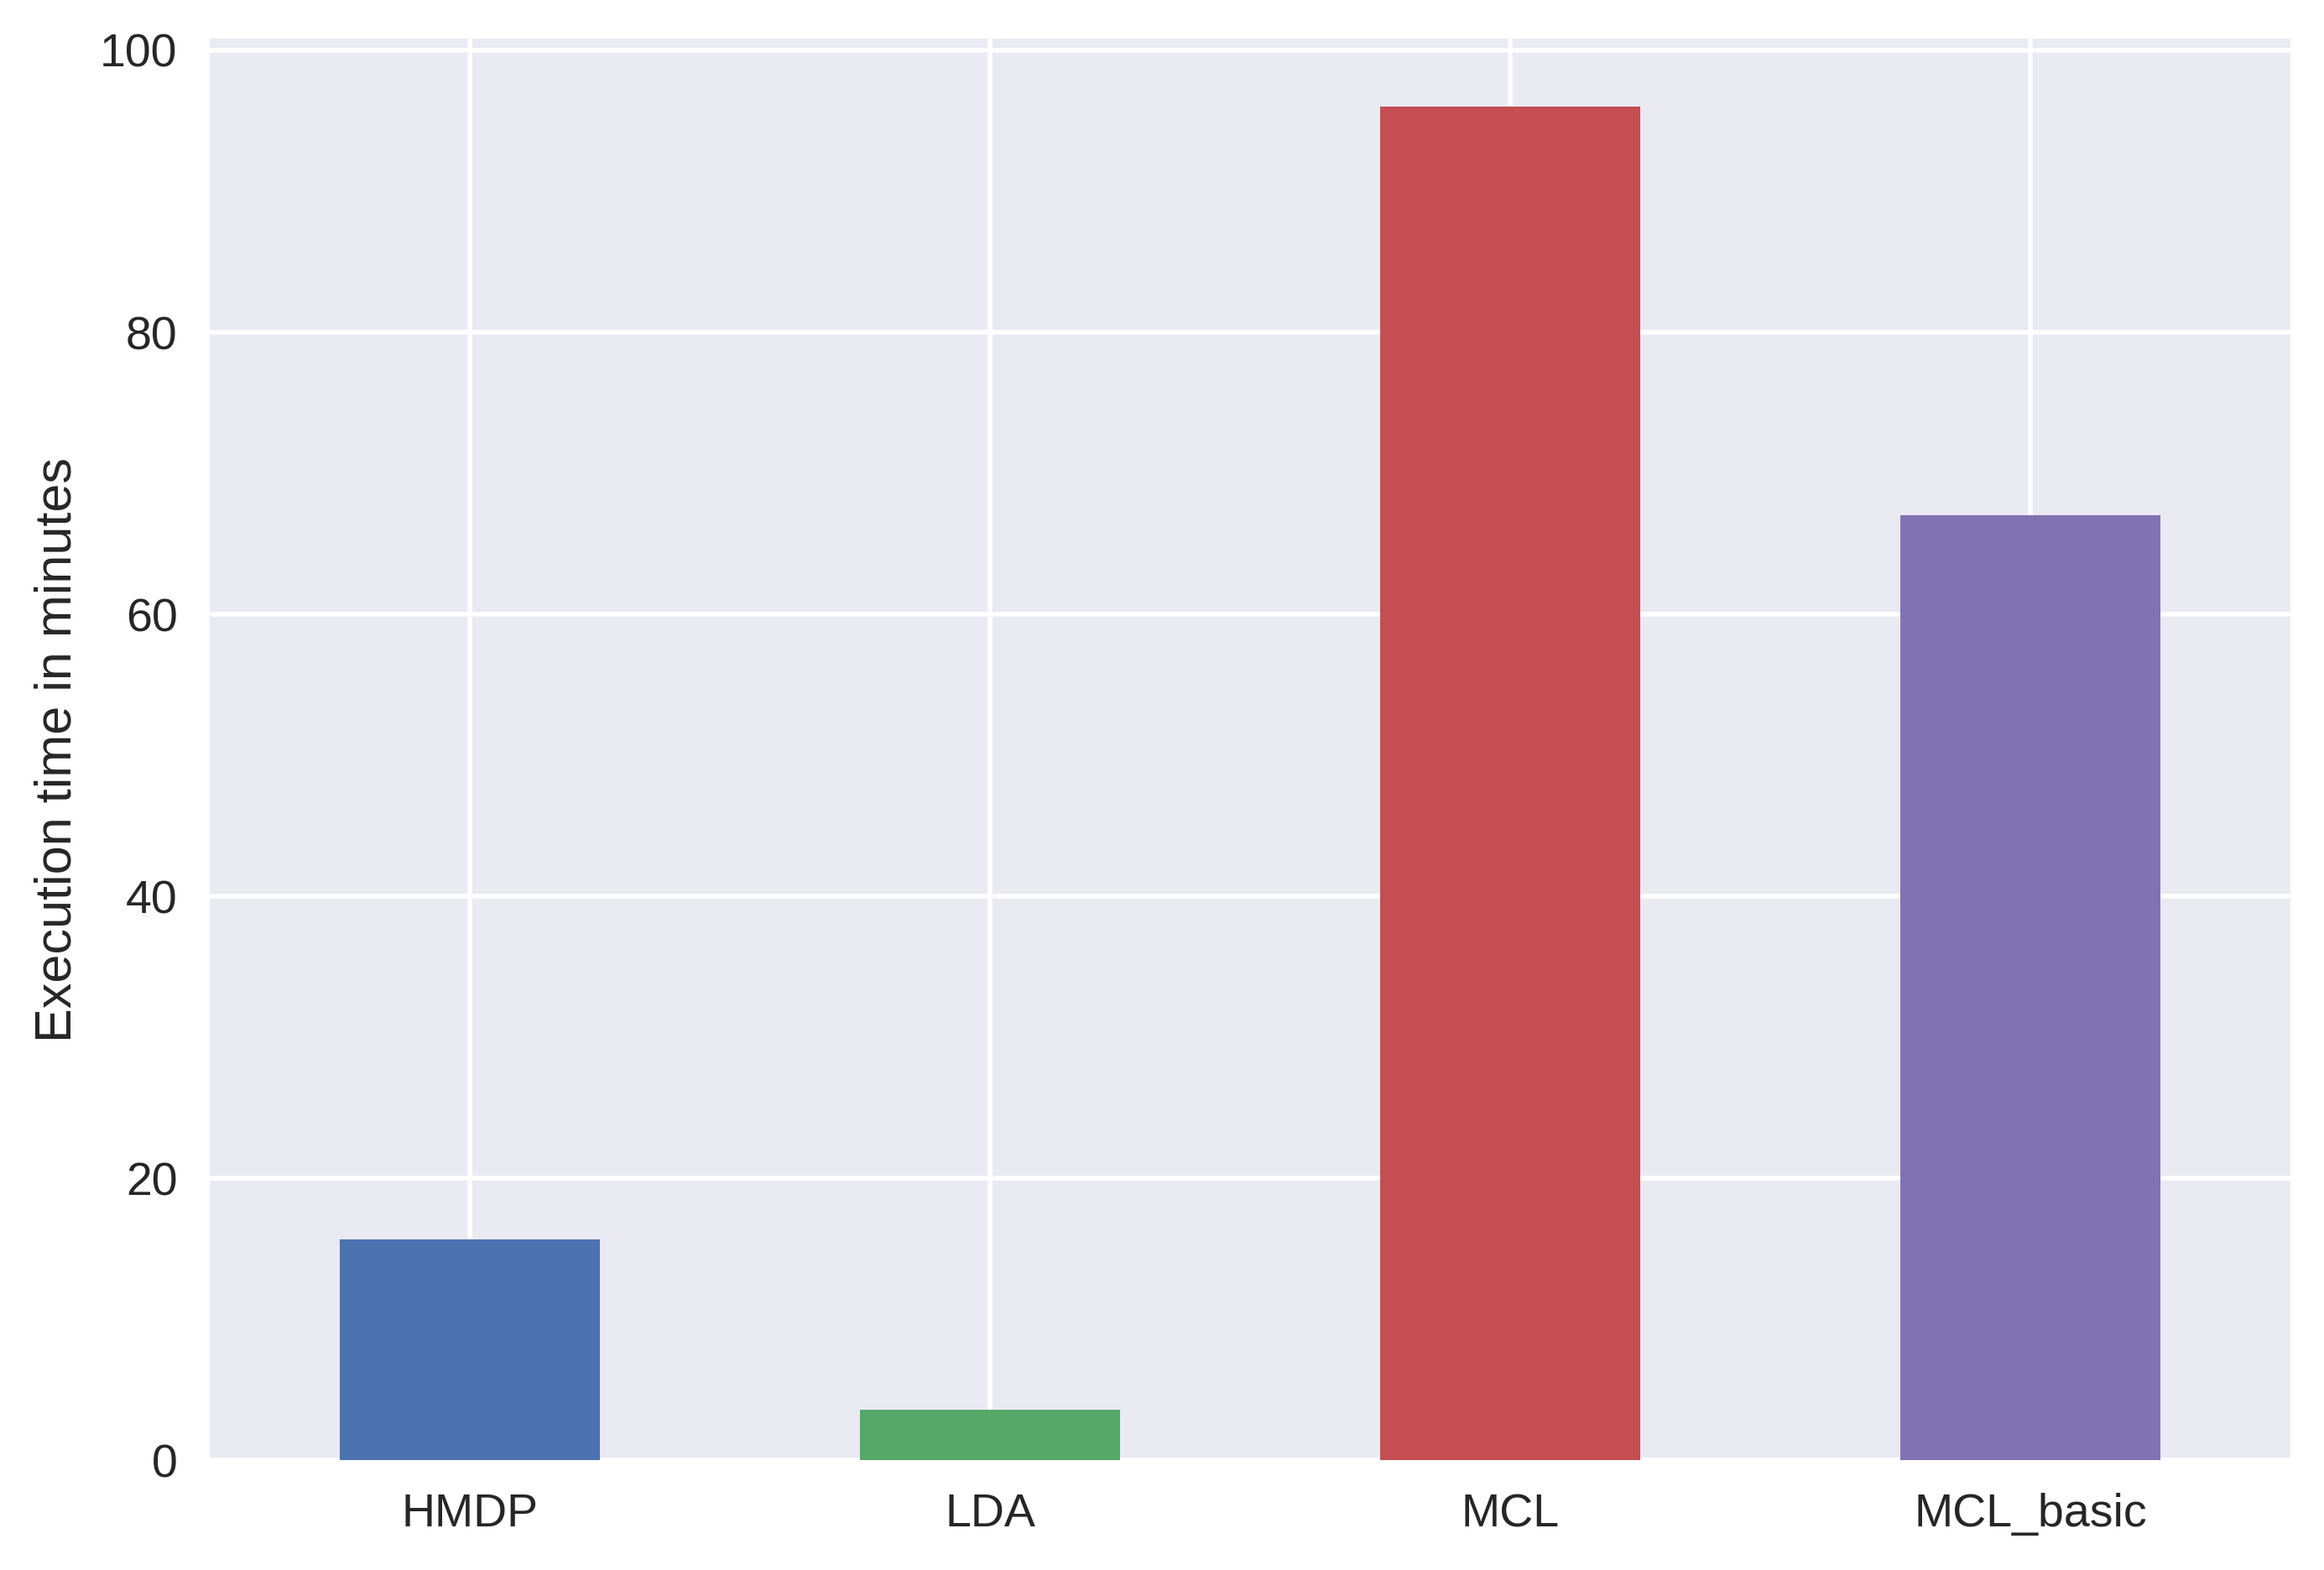
\includegraphics[height=2.8in]{img/exec_time_all_mts.png}%
\caption{Execution times of the different models on dataset \#3. Both MCL versions include graph build-up. MCL\_basic denotes the version with cosine similarity and thread-relationship and MCL the version as used in \cite{DBLP:conf/ecir/AkerKBPBHG16}. For HMDP and LDA words occuring 20 times or more were kept and the topic number restricted to 80.}
\end{figure}
A comparison of execution times on dataset \#3 shows that both topic models are faster than the MCL, which requires the similarity measurement of $\binom{n}{2}$ pairs of comments for graph build-up, which amounts to 19,185,915 pairs for 6195 comments.

\begin{figure}[H]%
\label{artthreads}
\centering
\subfigure[Boxplot of the no. of articles per topic]{%
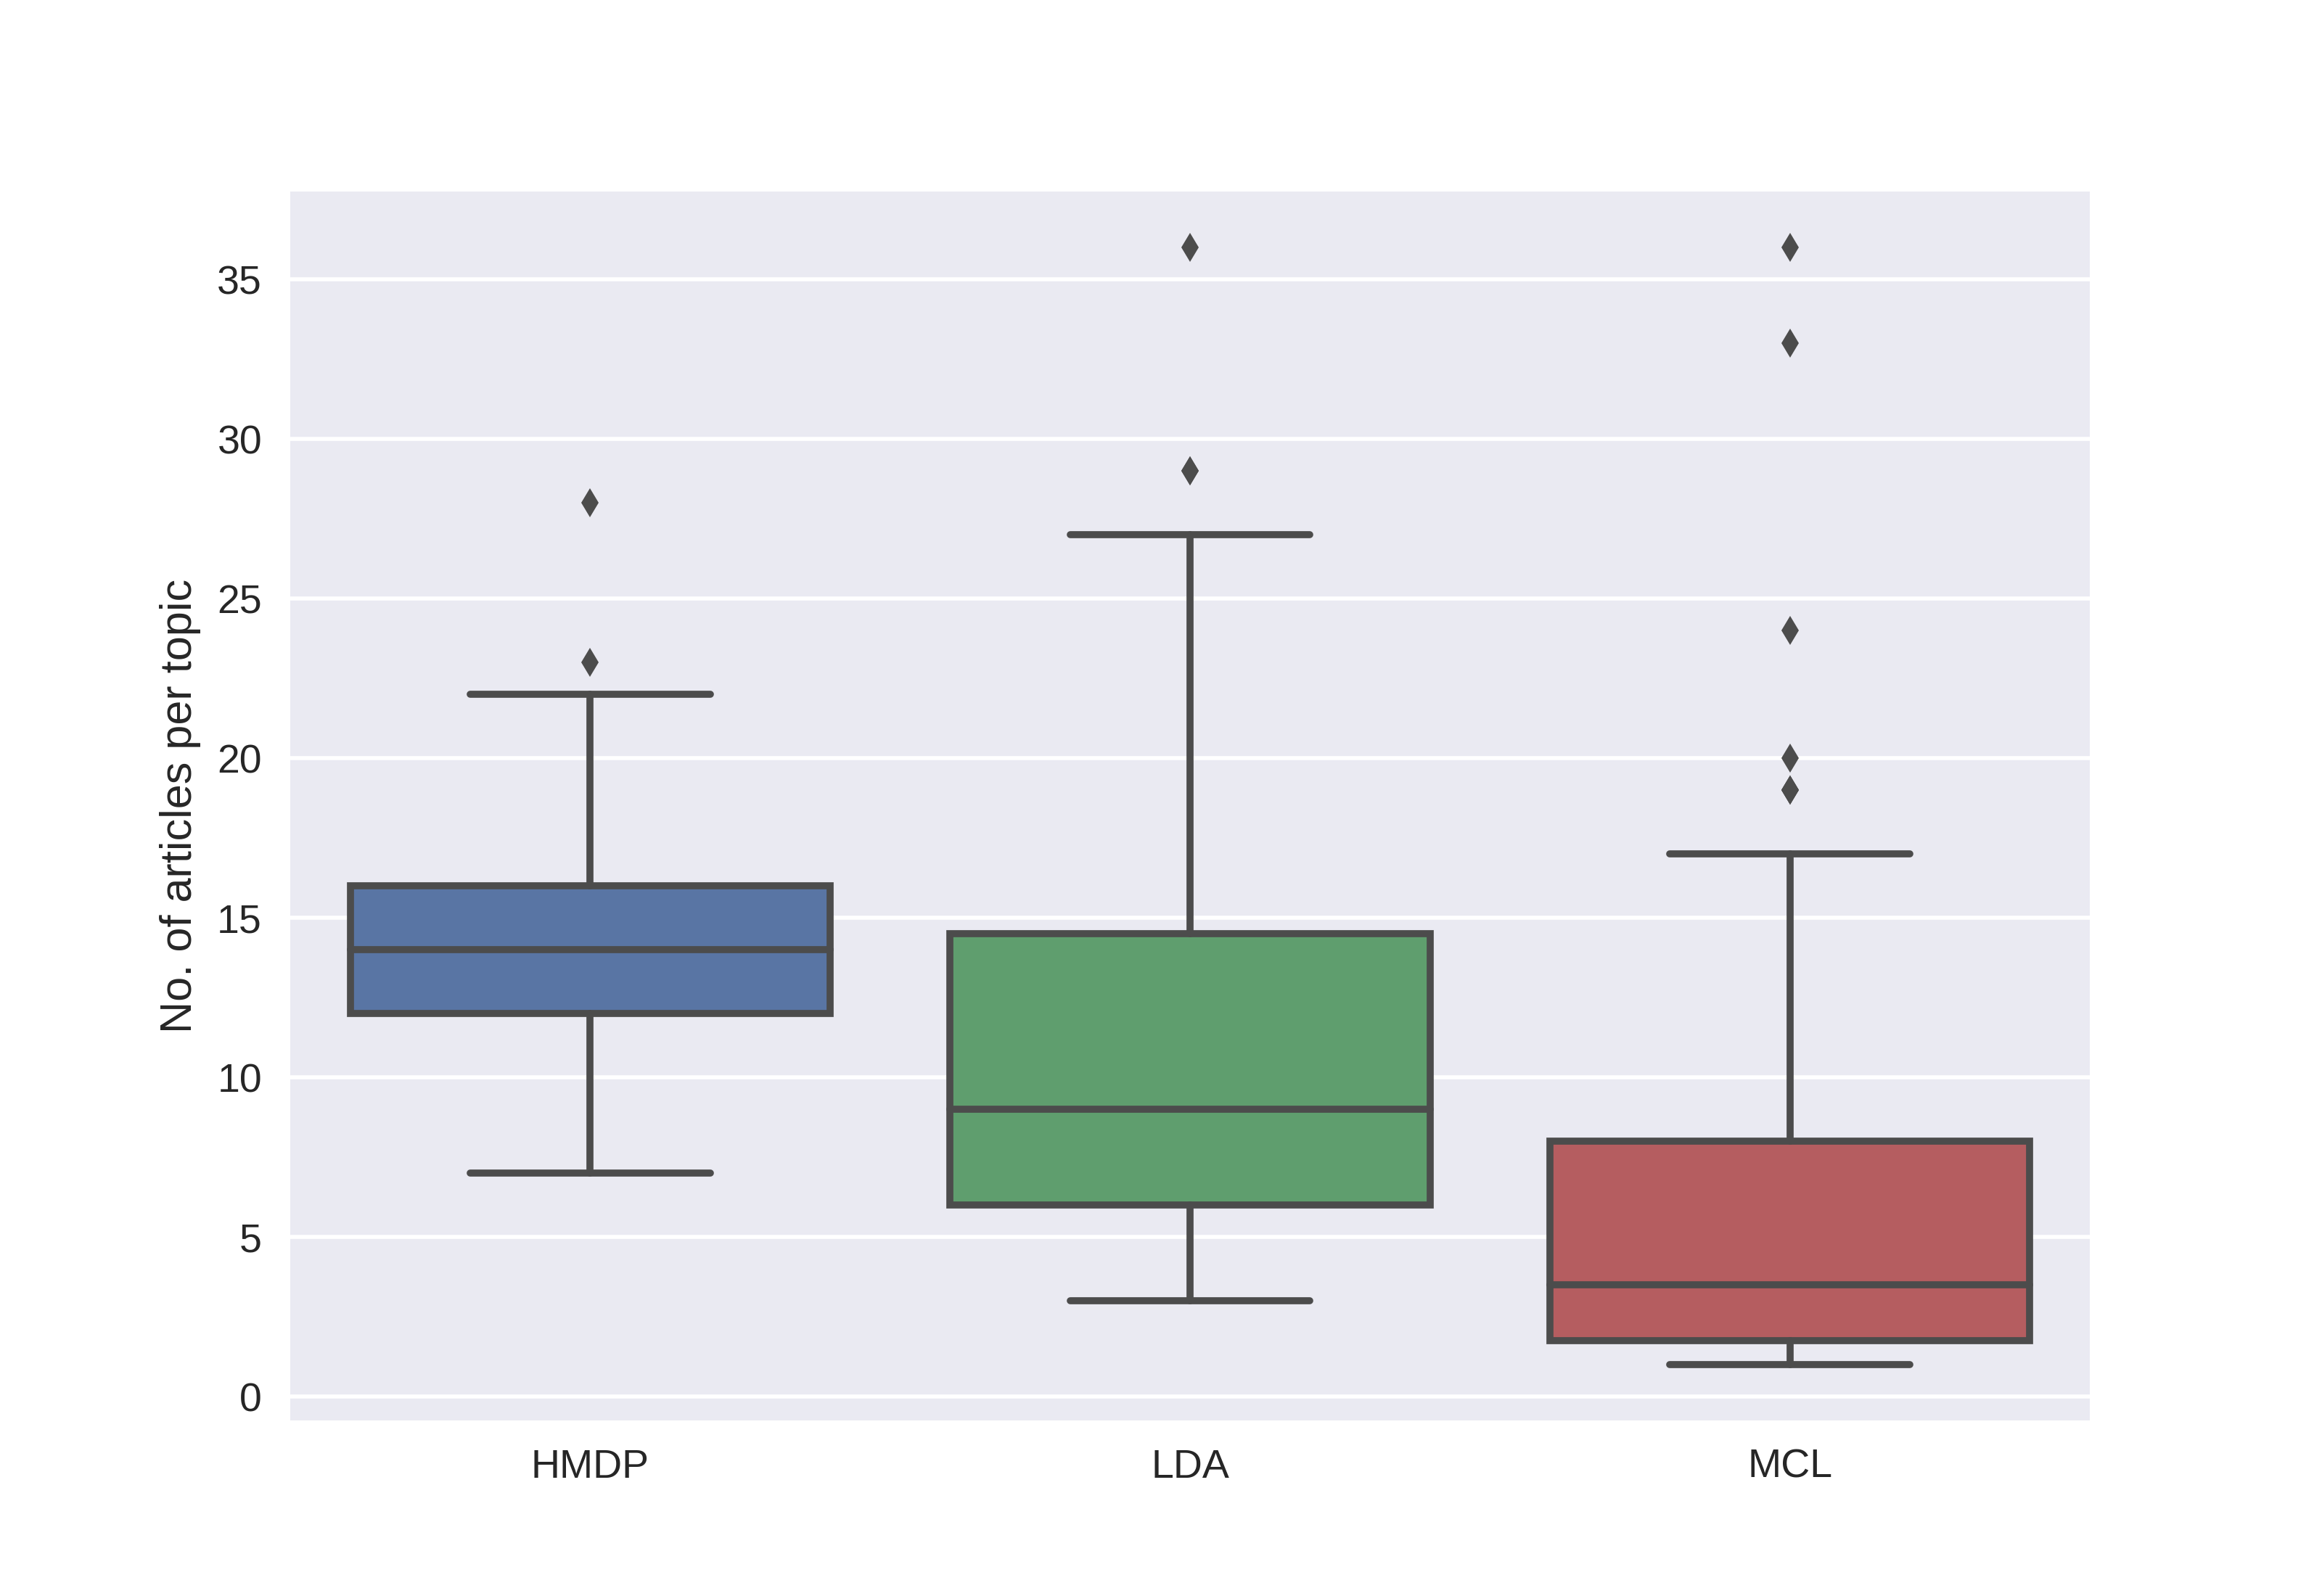
\includegraphics[width=0.75\textwidth]{img/articles_per_topic.png}}%
\qquad
\subfigure[Boxplot of the no. of threads per topic]{%
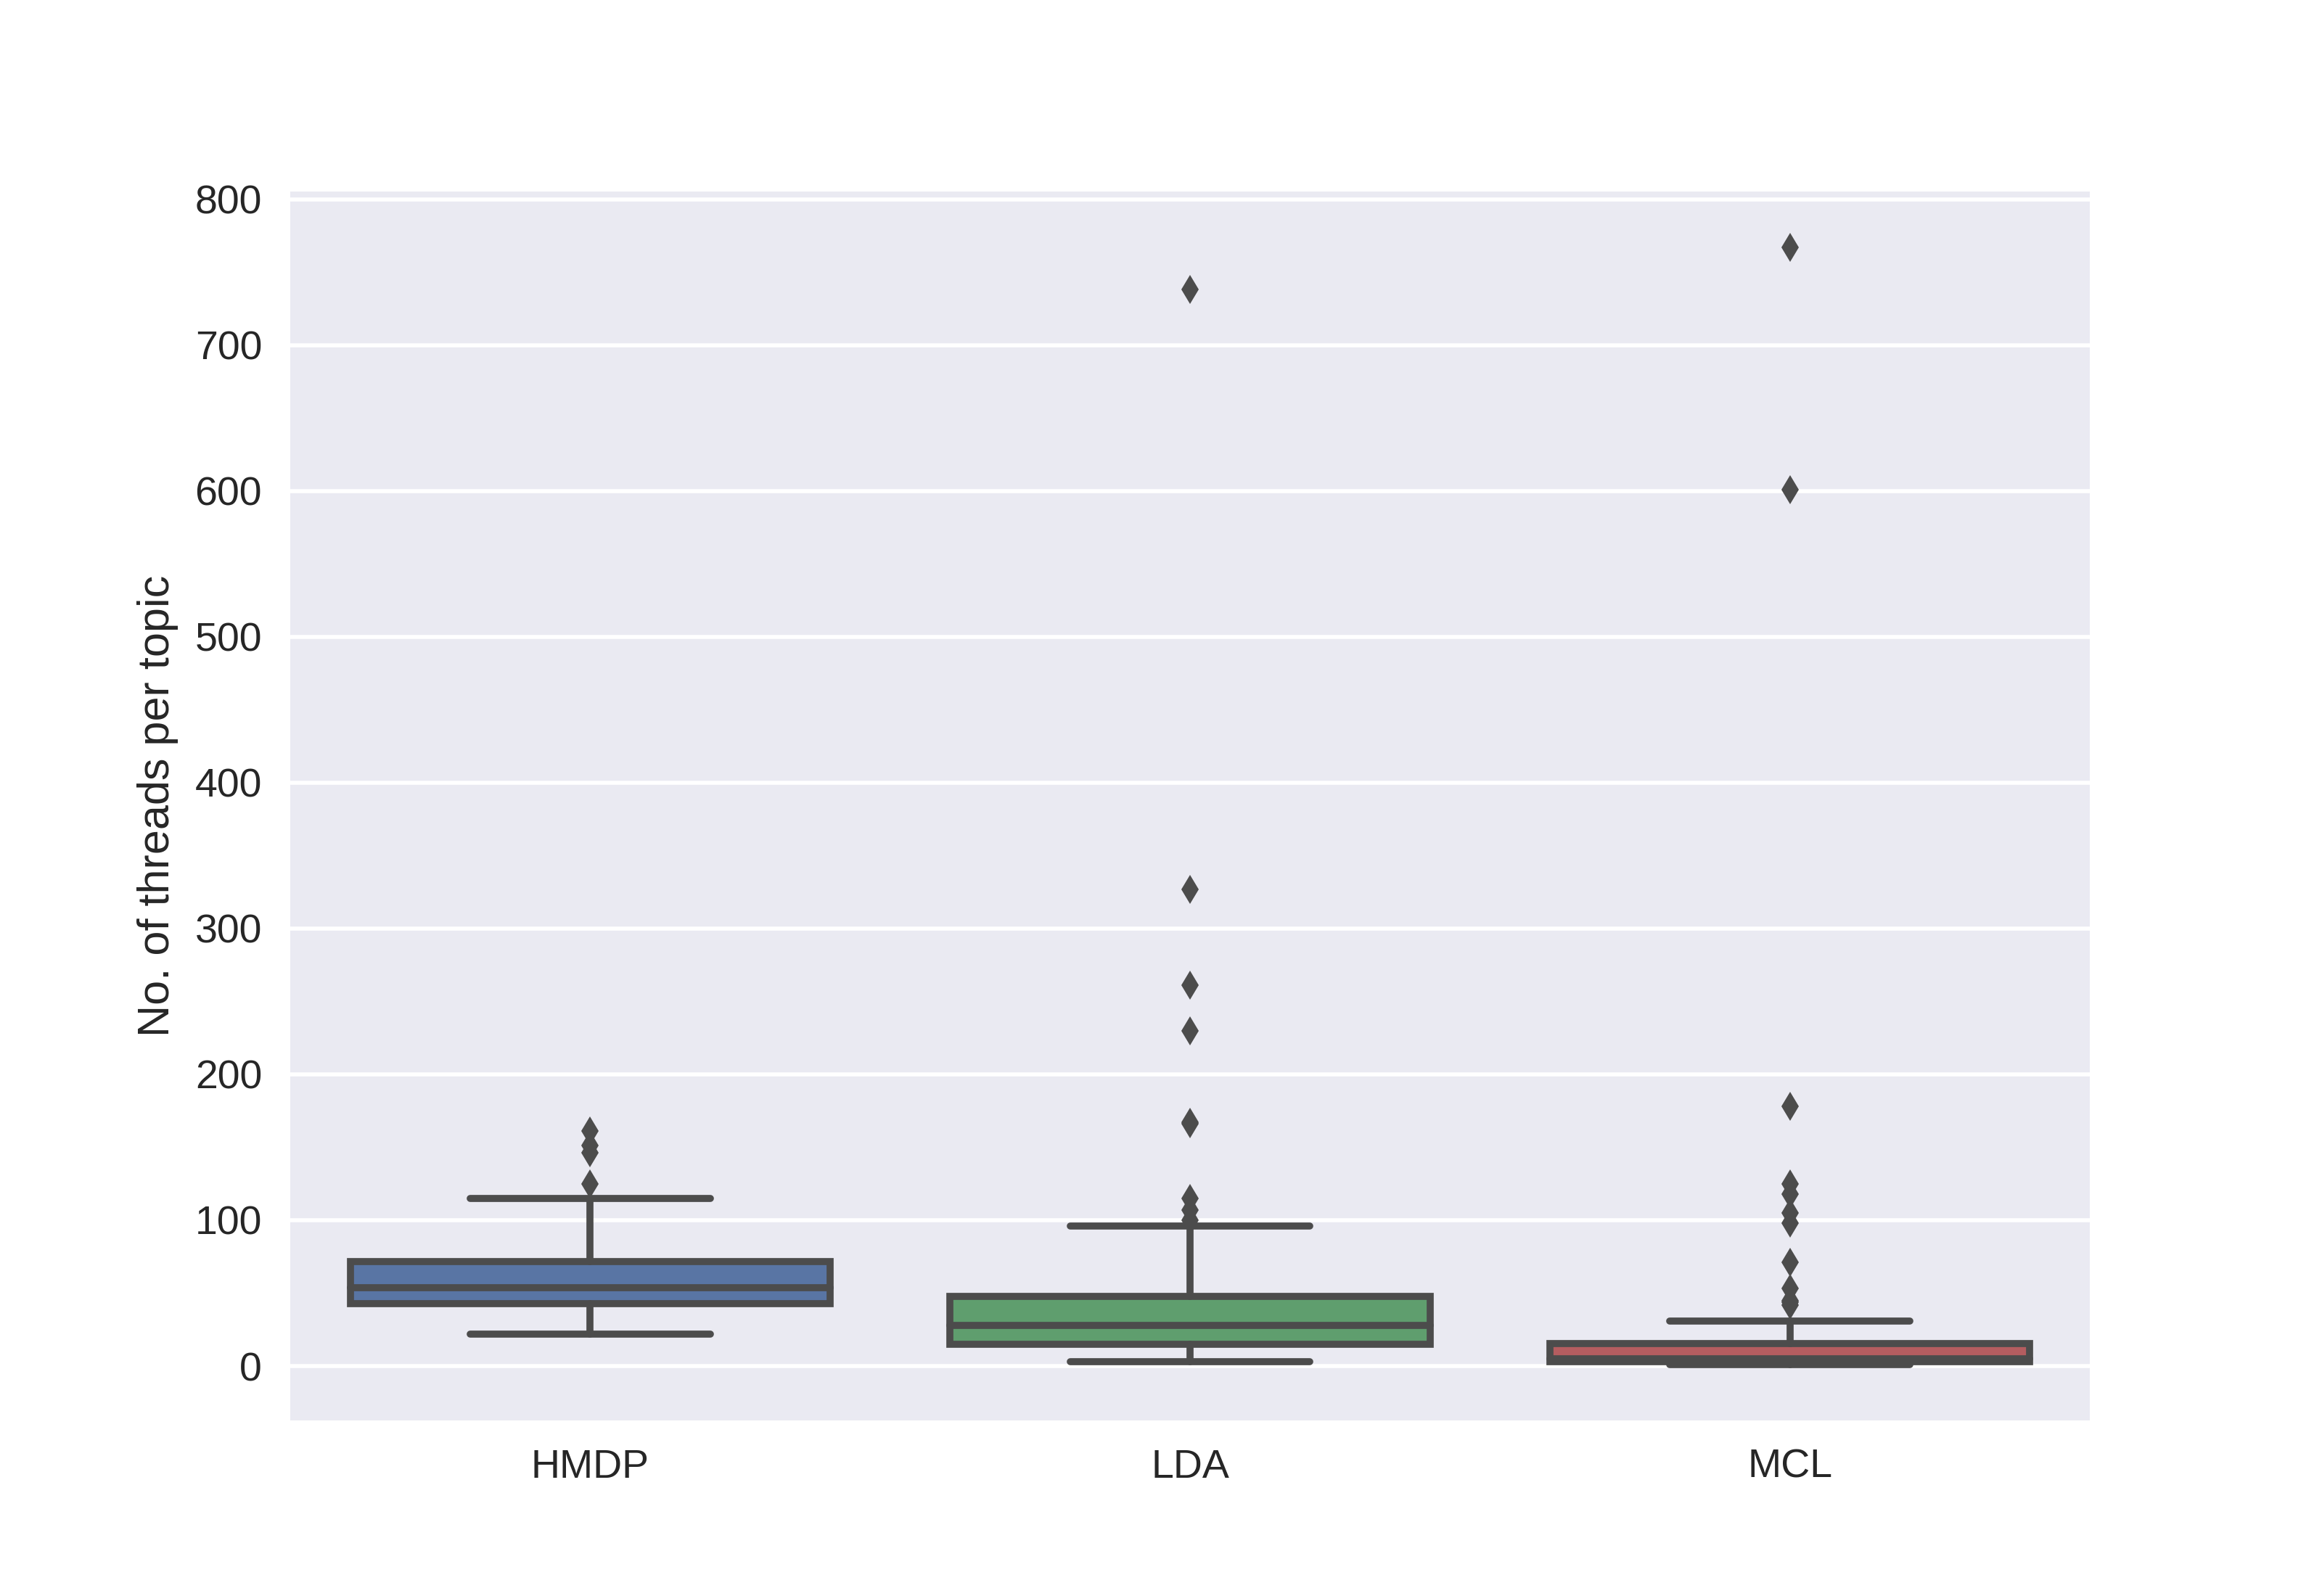
\includegraphics[width=0.75\textwidth]{img/threads_per_topic.png}}%
\caption{Description of the number of articles and threads contained in topic clusters found on dataset \#3. The number of topics / groups was restricted to 80.}
\end{figure}

\subsubsection{Comparison of HMDP and LDA}
\begin{figure}[H]%
\centering
\subfigure[Perplexity of HMDP and LDA on dataset \#1. Words occuring at least 2 times were kept.]{%
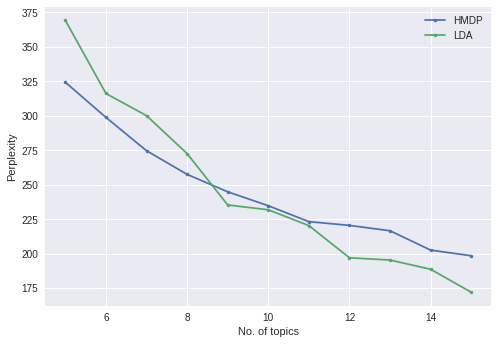
\includegraphics[height=2.8in]{img/perplexity_small2.png}}%
\qquad
\subfigure[Perplexity of HMDP and LDA on dataset \#3. Words occuring at least 30 times were kept.]{%
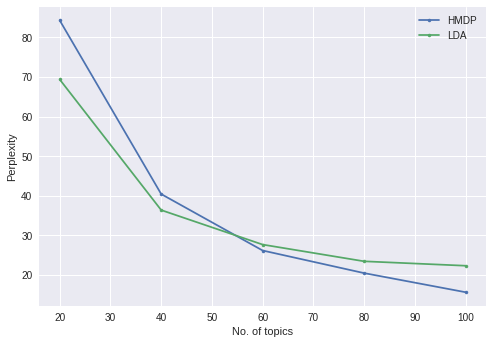
\includegraphics[height=2.8in]{img/perplexity_large2.png}}%
\caption{Perplexity of HMDP and LDA on datasets of different sizes. On both datasets 30\% of the documents were held-out for testing 70\% used for training.}
\end{figure}
HMDP and LDA do not differ greatly in terms of perplexity on all datasets.
\begin{table}[H]
\label{topicwords}
\centering
\begin{adjustbox}{max width=\textwidth}
\begin{tabular}{||c|c||}
\hline
HMDP & LDA \\[15pt]
\hline
\pbox{8cm}{wall border illeg build would hire work built employ mexico} & \pbox{8cm}{wall build built tunnel china fenc border street reduc hotel}\\[15pt]
\hline
\pbox{8cm}{white black student union organ group racist supremacist colleg univers} & \pbox{8cm}{student union colleg campu univers white ethnic member histor european} \\[15pt]
\hline
\pbox{8cm}{right ralli protest assault peopl free speech troubl person caus} & \pbox{8cm}{ralli protest assault speech shove event troubl attend crowd disrupt} \\[15pt]
\hline
\pbox{8cm}{black white live matter peopl dont racist say privileg race} & \pbox{8cm}{racism blm definit racist base race group superior belief discrimin} \\[15pt]
\hline
\pbox{8cm}{illeg alien tax money billion feder employ state dollar paid} & \pbox{8cm}{illeg cost dollar billion tax state level taxpay alien feder} \\[15pt]
\hline
\pbox{8cm}{muslim islam kill christian religion amal europ clooney sharia murder} & \pbox{8cm}{muslim christian islam terrorist thousand radic non gay rape death} \\[15pt]
\hline
\pbox{8cm}{women man men woman use bathroom room rape bruce transgend} & \pbox{8cm}{woman men women bathroom room bruce daughter molest transgend restroom} \\[15pt]
\hline
\pbox{8cm}{liber lie media left conserv truth brain dead wing agenda} & \pbox{8cm}{liber conserv speak polit left came realiz elect socialist today} \\[15pt]
\hline
\end{tabular}
\end{adjustbox}
\caption{Aligned subset of the 80 topics found out by HMDP and LDA on dataset \#3 outlined by the 10 most likely words by topic-word distribution.}
\end{table}
Comparison of the top words by topic-word distributions of HMDP and LDA shows that both find sensible and coherent topics across all datasets. \hyperref[topicwords]{The above table} illustrates inferred topics of dataset \#3, which is mainly concerned with the broad topic "Donald Trump" in the context of the general election 2016 in the United States of America.

\subsubsection{Context influence in HMDP}
\begin{figure}[H]%
\centering
\subfigure[Context influence on dataset \#1]{%
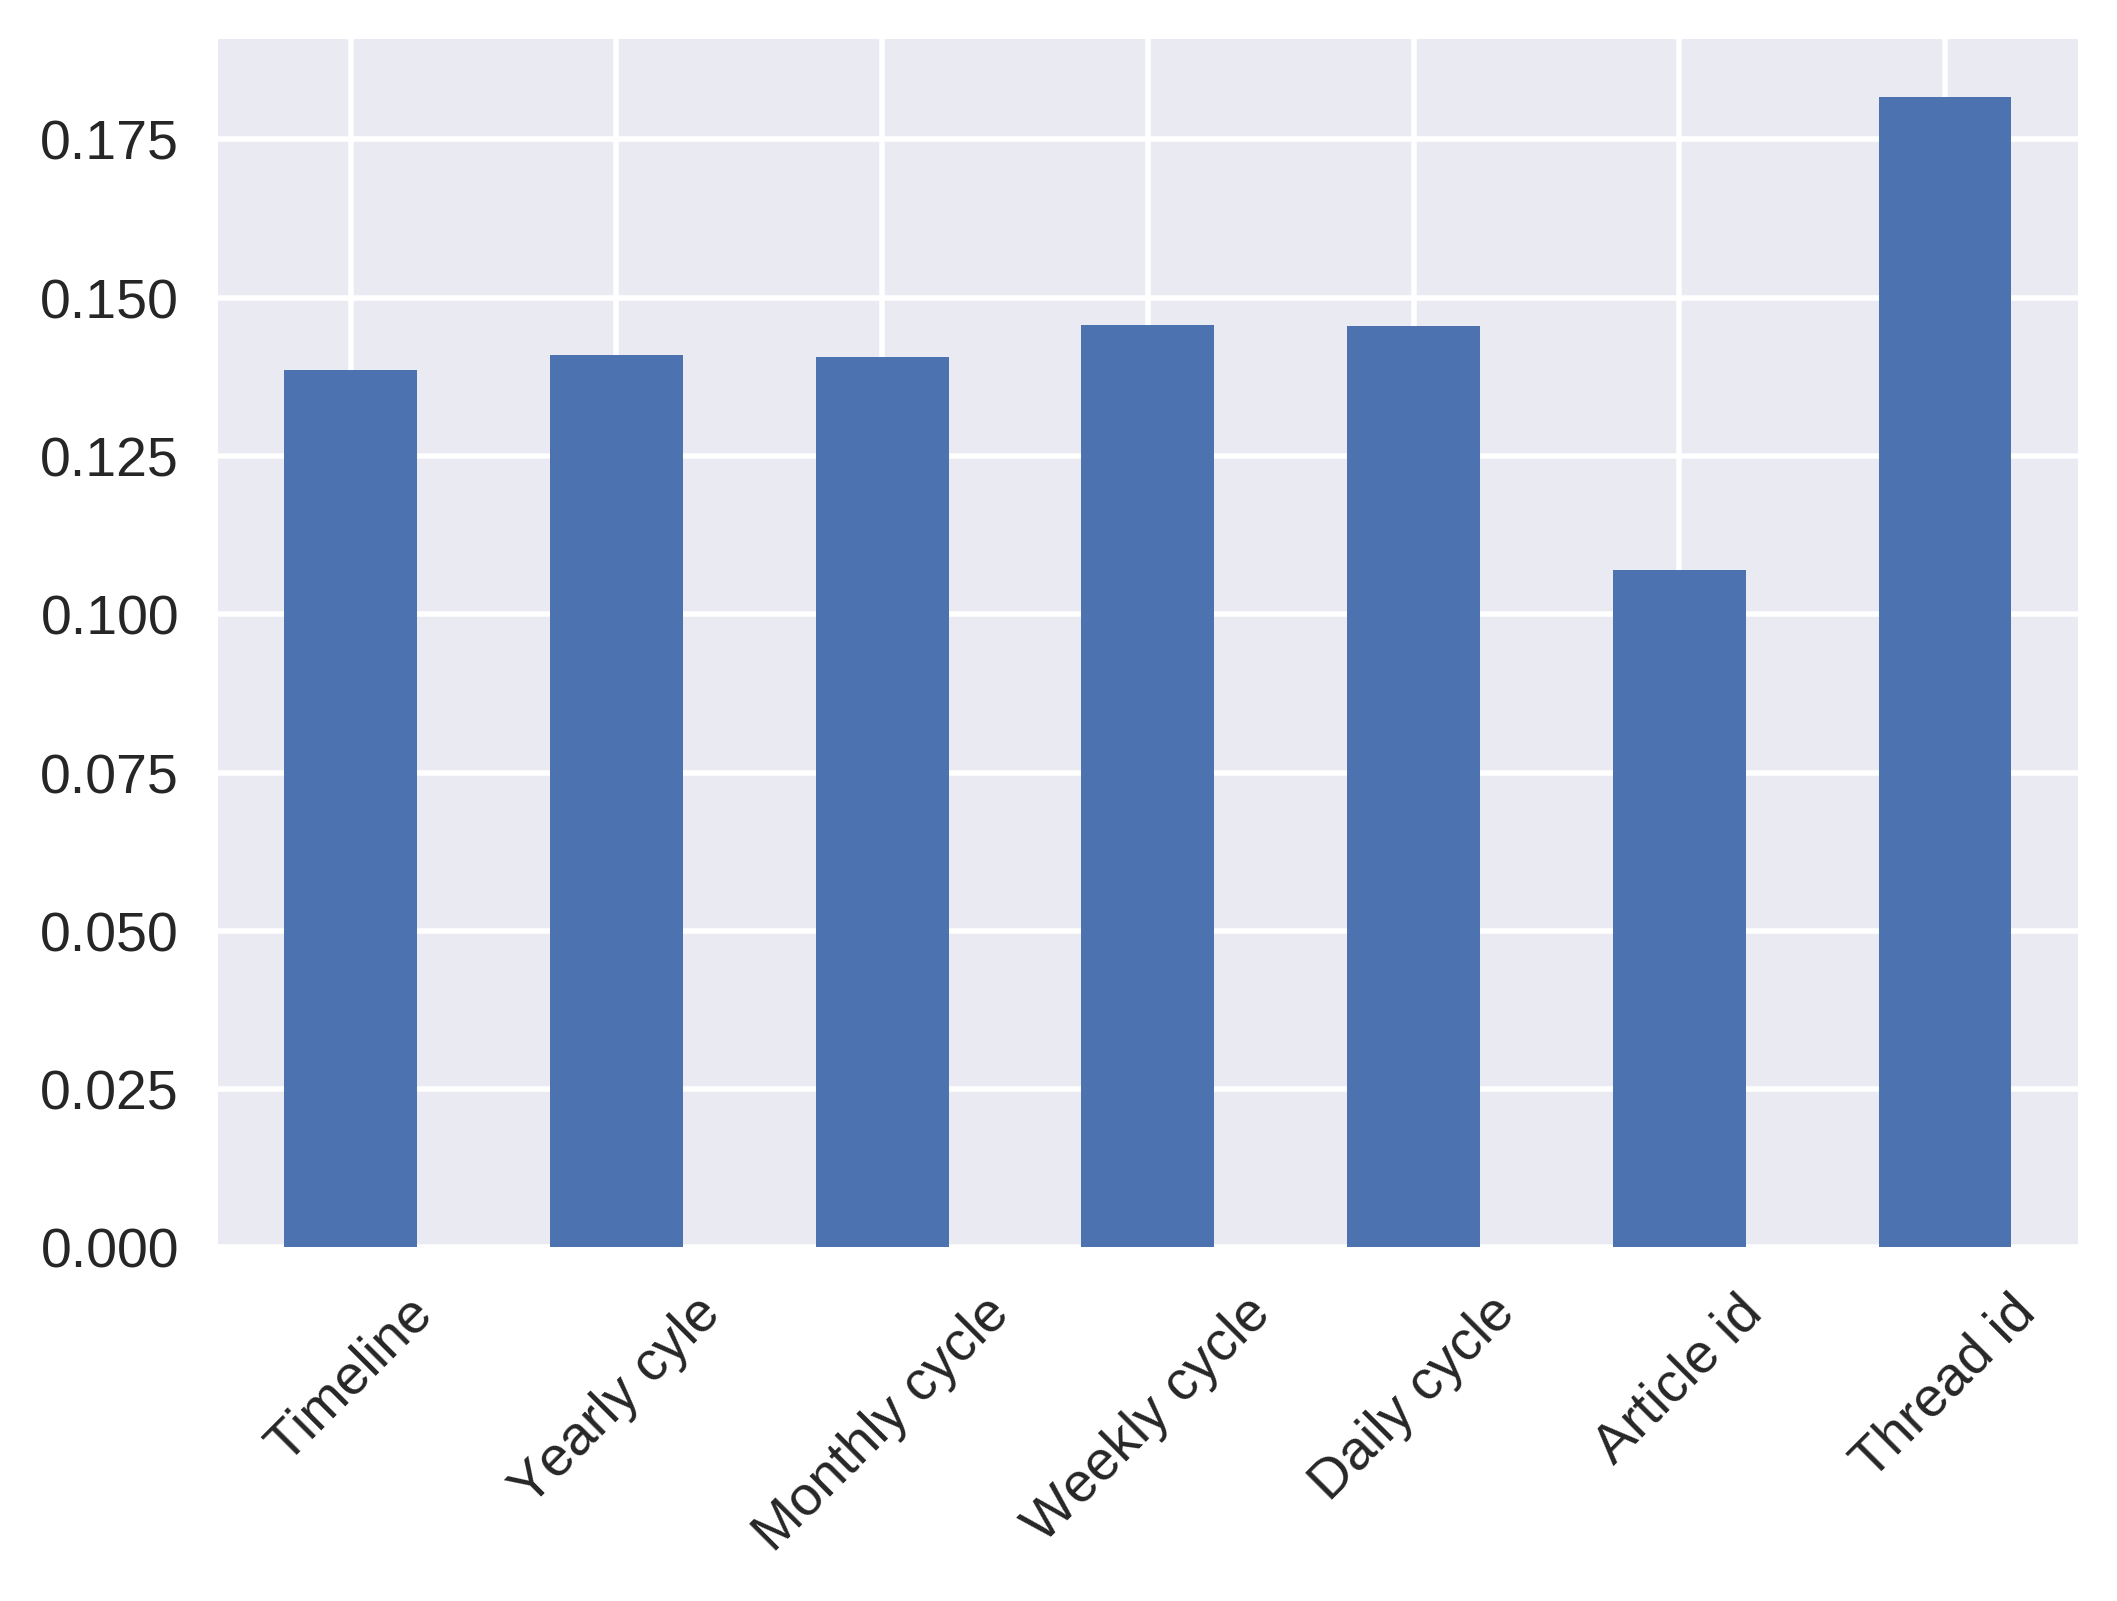
\includegraphics[height=2.8in]{img/context_weights_small.png}}%
\qquad
\subfigure[Context influence on dataset \#2 and \#3]{%
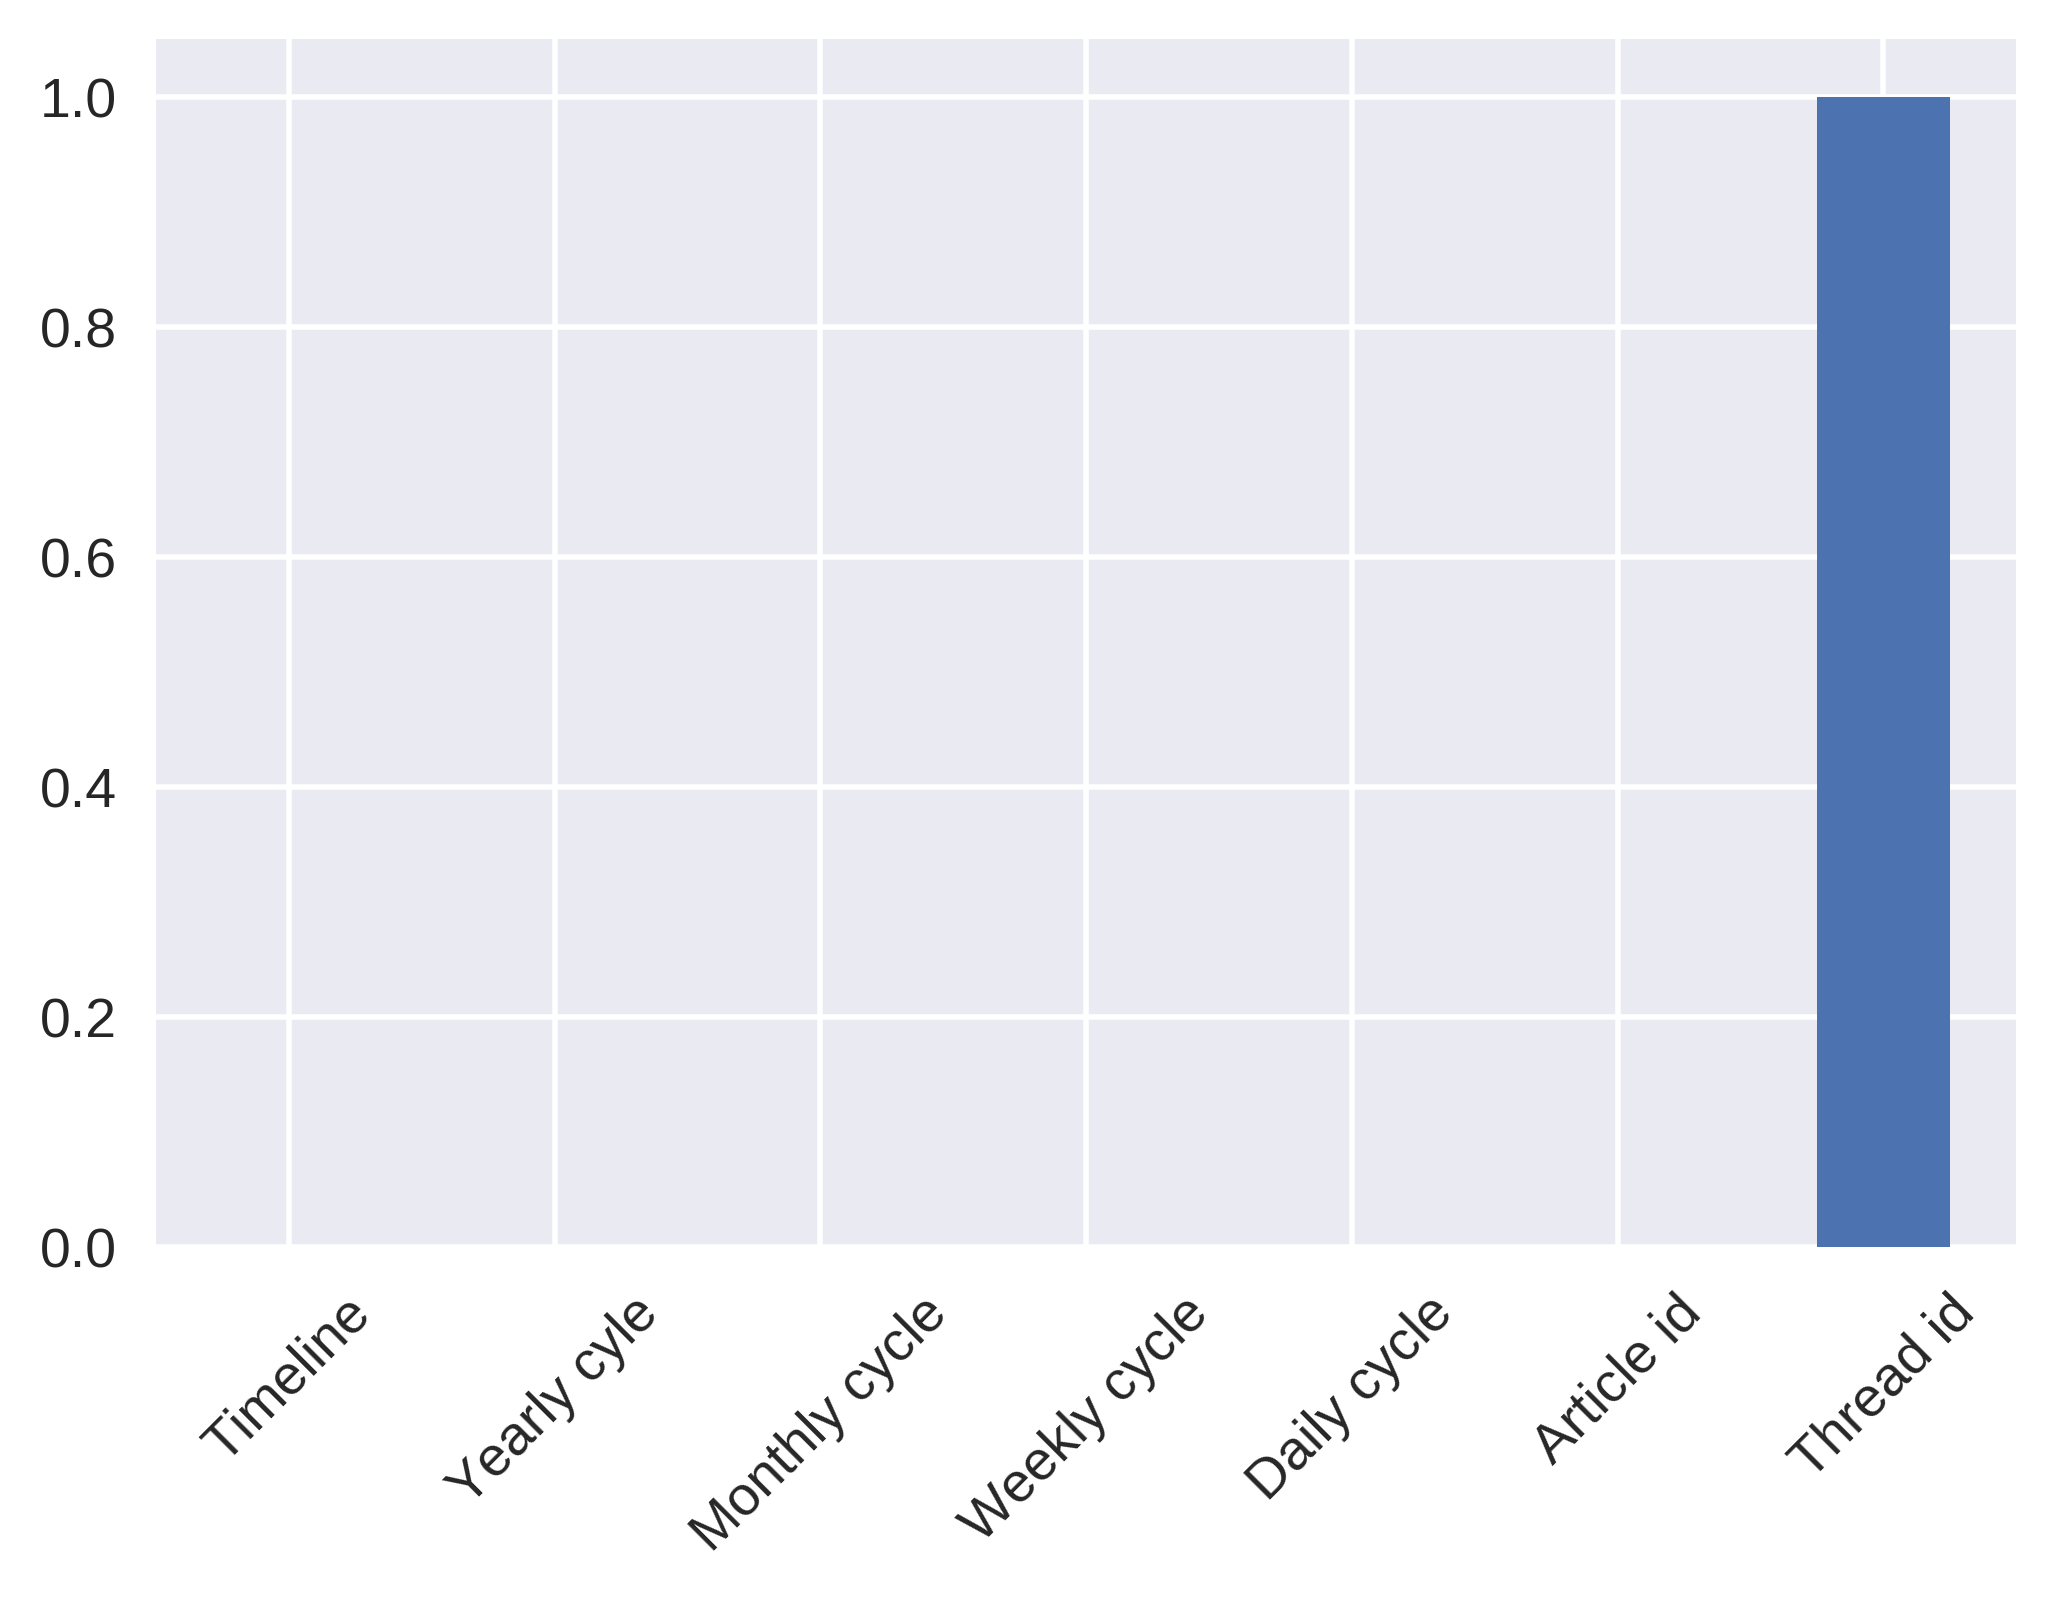
\includegraphics[height=2.8in]{img/context_weights_large.png}}%
\caption{Context space influence in the HMDP model.}
\end{figure}
In the HMDP model, the influence of each context space is stored in the variable $\zeta$ \cite{DBLP:phd/dnb/Kling16}. A higher context space weight is associated with a higher influence and indicativeness. The distribution of context weights is fairly smooth in the model trained on the small dataset \#1 with the thread-relationship being most influential. The thread-relationship is the sole influential form of metadata, when the HMDP is trained on the larger datasets \#2 and \#3.

\subsubsection{Topic labeling}
\begin{table}[H]
\begin{adjustbox}{max width=\textwidth}
\centering
\begin{tabular}{||c|c|c|c|c||}
\hline
Topic words & \#1 & \#2 & \#3 & \#4 \\[15pt]
\hline
\pbox{5cm}{wall border illeg build would hire work built employ mexico} & border wall & build wall & build border wall & great wall china \\[15pt]
\hline
\pbox{5cm}{white black student union organ group racist supremacist colleg univers} & white student & white student & white student union &  white student union \\[15pt]
\hline
\pbox{5cm}{right ralli protest assault peopl free speech troubl person caus} & speech right & trump rally & free speech right & going trump rally \\[15pt]
\hline
\pbox{5cm}{black white live matter peopl dont racist say privileg race} & black white & black lives &  black lives matter & black lives matter \\[15pt]
\hline
\pbox{5cm}{illeg alien tax money billion feder employ state dollar paid} & illegal aliens & state local & illegal aliens cost & state local level \\[15pt]
\hline
\pbox{5cm}{muslim islam kill christian religion amal europ clooney sharia murder} & christian islam & non muslims & muslim horde amal & 5 billion muslims \\[15pt]
\hline
\pbox{5cm}{women man men woman use bathroom room rape bruce transgend} & women men & mens room & man wearing women & according police report \\[15pt]
\hline
\pbox{5cm}{liber lie media left conserv truth brain dead wing agenda} & media lie & left wing & liberal left agenda & fit racial narrative \\[15pt]
\hline
\end{tabular}
\end{adjustbox}
\caption{Topic labels for HMDP topics infered on dataset \#3. The methods \#1 and \#3 used the approach outlined in \autoref{labeling} where the intersection of bi- / trigram and top topic words by topic word distribution was maximized. Columns \#2 and \#4 equal the most frequent bi- and trigram after stop word removal which is used as a baseline.}
\end{table}
The \hyperref[labeling]{presented algorithm} often yields descriptive labels with a sufficient amount of bi- and trigrams. Upon manual inspection, the labels generated by this approach are fairly similar to the labels found by the baseline approach using the most frequent bi- or trigram after stop word removal. Nevertheless, the baseline approach more often results in insensible labels such as "great wall china" in the first or "according police report" in the row before the last. Sometimes, however, the labels found by the approach outlined in \autoref{labeling} are also not completely descriptive of the topic such as in the row before the last where the labels indicate a topic about men and women and possibly clothing but fail to highlight that it is about the issue of transgender people and bathroom laws. Furthermore, noise in comments reduces the descriptiveness of the labels. Trigram labels appear to be more often descriptive than bigram labels, such as in the second row where "white student" fails to outline the problem of student unions which "white student union" does.
Furthermore, stop word removal seems to improve the quality of approaches \#2 and \#4 significantly but did not seem to have a strong effect on \#1 and \#3.

\subsection{Discussion}
The results show that the good results reported for the MCL version with seven similarity measures as reported in \cite{DBLP:conf/ecir/AkerKBPBHG16} could not be replicated. The thread-relationship of two comments was too influential and the clustering structure nearly mirrored the thread structure. Two differences between \cite{DBLP:conf/ecir/AkerKBPBHG16} and the presented thesis conceivably contribute to the different results. First and foremost, the domain of the works is different. While \cite{DBLP:conf/ecir/AkerKBPBHG16} targets the summarization of comments under a single article, this thesis aims to summarize comments under multiple articles. In the latter the conversational structure is broader, because topics not only overlap within comments of one article but of multiple articles. It is conceivable that a strong influence of the thread structure on clustering yields good results for summarizing comments under a single article, especially when threads under an article target fairly distinct topics, but less so for multiple articles. For multiple articles, a thread-heavy grouping appears unnatural as topics overlap across articles. On a different note, the regression model in this thesis differs from the one in \cite{DBLP:conf/ecir/AkerKBPBHG16}. Targets were obtained by a gold standard with target values of 0 and 1 and not by scraping comments quoting equal passages in an article with target values 0 for negative and in the range of 0.5 and 1 for positive samples. This might have contributed to a larger thread influence than in \cite{DBLP:conf/ecir/AkerKBPBHG16}. With a smaller thread-influence, as in the MCL which uses only cosine similarity and the thread relationship with weights of 1.7 and 0.1, the MCL resulted in a more natural grouping. In this setting it was compared to LDA and HMDP.
Here, we could reproduce the results of \cite{DBLP:conf/ecir/AkerKBPBHG16}, where the MCL outperformed LDA. Nevertheless, the MCL was surpassed in terms of F-measure and Precision by the HMDP. LDA was even surpassed across all measures. This comes to no surprise, since the context-aware generative model of the HMDP provides sounder model for comment creation, which is heavily influenced by context, than LDA. The improved results show the benefit of modeling context. The fact that the MCL, where such is indirectly included in the Markov graph build-up of the MCL, is able to outperform LDA corroborates this. The high precision of the HMDP indicates a higher topic separation compared to the other models. Especially, when compared to the MCL on the entire dataset \#3 this becomes apparent. MCL has a very high recall, but an observation of the cluster structure reveals nearly 75\% of the comments being clustered in the two largest clusters. This indicates that the MCL is less able to separate topics on a large set of comments. This might be explained by the effects of data sparsity in comments on similarity measurement. \par
As far as the approach chosen for evaluation is concerned, it is apparent that clustering an entire dataset but only measuring performance on an annotated subset is indicative. Still, it is limitated and requires thorough manual observation. A drawback of the method is the differing number of clusters between gold standard and inferred grouping, which likely results in a higher amount of false negatives. Therefore, using F$_{0.5}$-measure to emphasize precision over recall appears reasonable. \par
To conclude the model comparison, our results indicate that the HMDP provides the best performing model for the clustering of news article comments with an unknown number of discussed topics, for which modeling context was shown to be benificial. Furthermore, annotating a subset of a large dataset appears viable when results are manually observed, as well. 
\par In regards to topic model evaluation, the fact that BCubed-metrics clearly show a better performance of HMDP than LDA while Perplexity does not, highlights the restricted sufficiency held-out likelihood measurements for topic modeling evaluation. This has also been reported in studies such as \cite{NIPS2009_3700} and is an important conclusion for future work. Additional evaluation means than Perplexity, such as gold standard-based evaluation or user involvement as presented in \cite{NIPS2009_3700}, should be considered. \par
Coming back to the HMDP, the evaluation of metadata influence showed that the thread-relationship was most influential. This supports that its strong influence in the MCL as presented in \cite{DBLP:conf/ecir/AkerKBPBHG16} can be beneficial when summarizing a single article. Moreover, it supports the validity of the assumption that comments within a thread share a common topic. However, it is surprising that article-relationship and timestamp had no influence when the large corpus was modeled. For timeline influence, an explanation might be that there are too many overlapping topics at a certain time for the HMDP to find borders between context groups, especially in a broad topic domain. In a narrower topic domain, such as the small dataset \#1, the timely evolution of topics might be more substantial which is indicated by its associated context influence. The expected absence of cycles was corroborated. The significantly low influence of a comments article relationship might be explained two-fold. On the one hand, there might be too many articles which are closely related in terms of their topic to infer differences between comments from different articles. On the other hand, comments under an article might talk about too many different topics to be a sensible grouping. This would also support the idea that users bring in new information from related sources such as other articles or comments \cite{DBLP:conf/cikm/MaSYC12}. \par
Lastly, it could be outlined that our topic labeling approach outlined in \autoref{labeling} can produce descriptive labels when presented with a sufficient amount of data. However, the expressiveness of our results in cluster labeling is limited, since a formal evaluation of the labeling algorithm was not conducted.

\clearpage